% Primer Teorema de Isomorfismo
% Compilar con: pdflatex first_isomorphism.tex
\documentclass[tikz,border=10pt]{standalone}
\usepackage{tikz}
\usepackage{amsmath,amssymb}
\usepackage{xcolor}
\definecolor{gdlblue}{RGB}{41, 98, 168}
\definecolor{gdlred}{RGB}{191, 49, 49}
\definecolor{gdlgreen}{RGB}{30, 130, 76}
\definecolor{gdlorange}{RGB}{217, 130, 30}
\definecolor{gdlpurple}{RGB}{118, 56, 138}
\definecolor{gdlgray}{RGB}{140, 140, 140}
\definecolor{gdlyellow}{RGB}{190, 140, 10}
\usetikzlibrary{arrows.meta, positioning, shapes.geometric}

\begin{document}
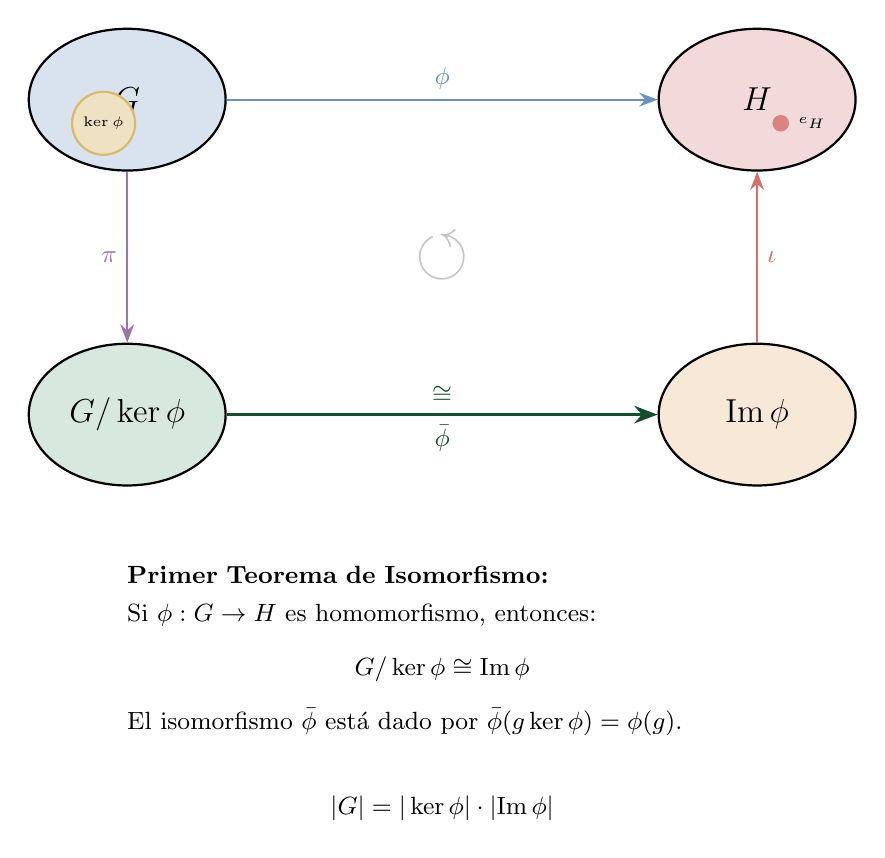
\begin{tikzpicture}[
    >=Stealth,
    group/.style={ellipse, draw, thick, minimum width=2.5cm, minimum height=1.8cm, font=\large},
    arrow/.style={->, thick}
]

% === Grupos ===
\node[group, fill=gdlblue!18] (G) at (-4, 2) {$G$};
\node[group, fill=gdlred!18] (H) at (4, 2) {$H$};
\node[group, fill=gdlgreen!18] (GK) at (-4, -2) {$G/\ker\phi$};
\node[group, fill=gdlorange!18] (Im) at (4, -2) {$\mathrm{Im}\,\phi$};

% === Flechas ===
% φ: G → H
\draw[arrow, gdlblue!70] (G) -- node[above, font=\small] {$\phi$} (H);

% Proyección canónica π: G → G/ker(φ)
\draw[arrow, gdlpurple!70] (G) -- node[left, font=\small] {$\pi$} (GK);

% Inclusión Im(φ) ↪ H
\draw[arrow, gdlred!70] (Im) -- node[right, font=\small] {$\iota$} (H);

% Isomorfismo inducido
\draw[arrow, very thick, gdlgreen!60!black] (GK) -- node[below, font=\small] {$\bar{\phi}$} node[above, font=\small] {$\cong$} (Im);

% === Kernel ===
\begin{scope}[shift={(-4, 2)}]
    \draw[thick, fill=gdlyellow!25, draw=gdlyellow!60] (-0.3, -0.3) circle (0.4cm);
    \node[font=\tiny] at (-0.3, -0.3) {$\ker\phi$};
\end{scope}

% === Elemento de identidad en H ===
\begin{scope}[shift={(4, 2)}]
    \fill[gdlred!60] (0.3, -0.3) circle (3pt);
    \node[font=\tiny, right] at (0.4, -0.3) {$e_H$};
\end{scope}

% === Diagrama conmutativo ===
\node[font=\Huge, gdlgray!50] at (0, 0) {$\circlearrowleft$};

% === Etiquetas ===
\node[font=\small, text width=8cm] at (0, -5) {
    \textbf{Primer Teorema de Isomorfismo:}\\[0.3em]
    Si $\phi: G \to H$ es homomorfismo, entonces:
    \[G/\ker\phi \cong \mathrm{Im}\,\phi\]
    El isomorfismo $\bar{\phi}$ está dado por $\bar{\phi}(g\ker\phi) = \phi(g)$.
};

% Fórmula adicional
\node[font=\small] at (0, -7) {
    $|G| = |\ker\phi| \cdot |\mathrm{Im}\,\phi|$
};

\end{tikzpicture}
\end{document}
